\chapter{毫米波蜂窝系统基站天线资源分配与优化研究}

\textbf{本章摘要:} 本章以下一代蜂窝网络为背景研究星型网络结构下的毫米波通信资源优化问题。在上一章工作给出了小区内多个用户位置信息的基础上,研究如何分配基站上天线阵列资源以最大化系统收益即系统吞吐量的问题。在毫米波蜂窝网络中,基站上的大规模天线阵列虚拟地分成若干个均匀线性子阵列,通过波束成形技术与对应用户进行通信。由于大规模天线阵列与每个均匀线性子阵列都有着固定的形状,因此问题建模为如何在资源有限的矩形阵列中选择并合理地放置这些子阵列,使得系统收益最大,这既需要考虑每个子阵列的天线数量,又需要考虑这些子阵列在矩形天线阵列中的位置分布。针对不同的子阵列放置方式又包含两种不同情况:1)所有线性子阵列都互相平行且平行于矩形阵列的一条边;2)为了进一步提高系统收益,线性子阵列可以平行于矩形阵列的任意一条边,即存在相互垂直的子阵列。分别考虑两种情况并对问题建模,针对两个NP-hard问题,将每种情况都进行分解并逐步解决每个子问题。通过解决一系列的多选择背包问题、多背包问题和带状装箱问题,得到了两种情况下的多项式时间近似算法,并给出了每个算法的计算复杂度和理论下界。仿真结果证明了提出的两种算法在不同的情况下都能有效地分配天线资源,得到有性能保证的系统收益。

\textbf{关键词:}毫米波通信;Massive MIMO;整数规划
%\keywords{毫米波通信;Massive MIMO;整数规划}

\section{引言}
近几十年,移动通信技术发展日新月异,从上世纪八十年代出现的以GSM和CDMA为标志的2G技术开始,再到WCDMA,CDMA2000以及我国提出的TD-SCDMA并行的3G技术的发展,进而到近些年以OFDM和MIMO为核心的4G技术,移动通信技术正在经历着相当快速的发展。在最新的长期演进技术升级版(Long Term Evolution - Advanced, LTE-Advanced)技术中,通信的峰值速率已经可以达到100MHz的带宽,下行速率可达1Gbps,上行可达500Mbps。
随着人类与社会对移动通信的需求的提升,尤其是近些年高清视频、即时通信与物联网(Internet of Things, IoT)等应用的发展,现有的移动网络无论是在连接速度、通信延迟还是接入数量都渐渐难以满足需要。因此针对下一代移动通信技术,即5G技术的研究就迫在眉睫。一般认为\cite{andrews2014will},5G蜂窝通信将会在2020年到来,为人们带来1000倍的系统容量增加,10到100倍的链接数量和终端速率提升,5倍的延迟降低以及针对那些低电量设备的10倍的电池寿命延长。当然,这些要求并不是要在所有情况下同时满足,例如在高清流媒体视频播放时,更高的传输速率的重要性就远远超过了低延迟和系统可靠性等保障。与此相反的是在无人驾驶等领域,系统的低延迟和可靠性必须优先保证,而对传输速率的要求则可以适当放宽。

性能的提升必须要求技术上的巨大突破。一般认为,下一代移动通信系统主要将从毫米波通信\cite{noh2016zero,li2016optimizing},Massive MIMO\cite{araujo2016massive},致密化小区\cite{qian2017joint}(Extreme Densification),全双工通信(Full Duplex Radio),设备到设备通信(D2D Communication)等技术中进行突破。其中致密化小区,毫米波通信、波束成形技术与大规模多输入多输出技术被认为是最重要的核心技术手段。
事实上,这些技术的关系是相辅相成的。毫米波通信应用的主要难点在于在毫米波频段上,无线电波在空间中衰减得很快\cite{sulyman2014radio}。因此,基于大规模多输入多输出技术的波束成形技术正合适利用于此。此技术可以将毫米波信号集中在一个非常窄的波束上,能够极大的提高信号的传输效率\cite{li2009robust,roh2014millimeter}。首先由于毫米波信号的传输性质,一个基站所能通信的范围大大地缩小,对通信范围外的干扰也会显著降低,这恰巧符合超致密化小区的要求,提高了频谱利用率。 一方面,传统的厘米波段的通信要求相对大的天线尺寸及天线间空隙,因此难以将天线阵列部署在移动端;而毫米波的使用能够极大地减小天线单元的体积以及天线之间的空隙,进而减小整个天线阵列的体积,从而使得将大规模天线阵列布置在移动端成为可能。另一方面,只有通过基于大规模阵列天线的波束成形技术,才能将本身极易衰减的高频毫米波信号通过高方向性的能量集中的波束进行传输,进而提高频谱的利用率。通过利用波束成形技术,在发射或者接收端使用更多的天线意味着能量传输更加的集中。因此,由此而生的问题便是当基站可用天线数量一定的情况下,如何通过合适的基站天线-用户分配,使整个通信系统收益最大。在本章中将选取系统吞吐量这一最具代表性的系统收益进行分析。

\begin{figure}[t]
\centering
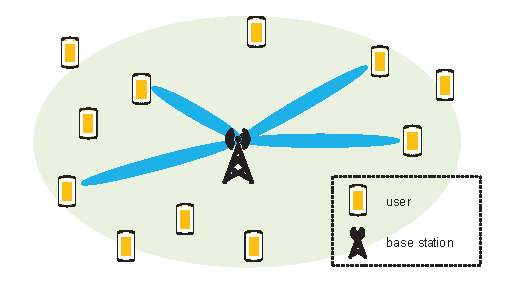
\includegraphics[width=0.7\textwidth]{Pictures/M-1.pdf}
\caption{毫米波蜂窝网络系统示意图}
\label{fig:0}
\end{figure}

波束成形技术主要有以下三种,即模拟波束成形,数字波束成形以及混合模拟数字波束成形技术。数字波束成形技术实现在基带阶段,将计算好的信号相位和幅度通过一个单独的射频链传输到一个天线上。这种方法能够达到系统最优容量,但是其计算消耗以及能量消耗也非常巨大,同时由于每个天线都需要一套昂贵的数模/模数转换器,因此难以将其实现在大规模天线阵列当中\cite{doan2004design}。另一方面,模拟波束成形技术\cite{wang2009beam}是实现在天线阵列中的一个射频链和基带上,只控制与之相连接的一组天线终端的相位,进而能够集中信号发射能量并形成一个窄波束。模拟波束成形技术相较于数字波束成形,能够大幅减少计算复杂度,同时减少系统整体价格,尽管会有一定的系统性能降低。因此,有学者提出融合两种算法优点的混合模拟数字波束成形技术。混合波束成形技术在基带上使用数字波束成形技术,每个基带连接到一个射频链上,每个射频链连接到一个由一组天线终端构成的\emph{子阵列}上。模拟波束成形技术就运用在该子阵列上。这种组合是的波束成形技术更加有效更加实际地运用在毫米波大规模多输入多输出天线阵列通信中。至此的问题变成如何通过选择合适的子阵列以提高系统的吞吐量。

考虑在毫米波下行通信中的基站天线子阵列选择问题,使用均匀线性阵列(Uniform Linear Array, ULA)作为基本的子阵列与一个用户进行通讯。因此任务就是如何合适地将整个矩形天线阵列分割成若干个均匀线性阵,使得总的系统吞吐量最大化。在这其中考虑两种情况,首先考虑当所有的子阵列都按照同一个方向排列时的情况,即所有均匀线性阵都相互平行,将该子阵列选择问题建模成一个非线性$0-1$整数规划问题。由于要同时优化每个子阵列的天线数量以及其在天线阵列中的位置,因此问题很难求解。首先将原问题分解成一个多选择背包问题(Multiple Choise Knapsack Problem, MCKP)和一个多背包问题(Multiple Knapsack Problem, MKP)。之后利用一个完全多项式时间解法(FPTAS)来解决MCKP问题,并基于MCKP问题的结果使用启发式算法解决了MKP问题。最后的结果可以证明与理论最优解之间的差可以限制在$1/2(1-\epsilon)$最优解的界中。此外还解决了第二个情况,即子阵列按照两种互相垂直的方向排列在天线阵列中,两个子阵列之间可以是相互平行的或是相互垂直的。这种情况提高了子阵列选择的自由度,但是也使得问题更加难以求解。相类似,将原问题转化为一个MCKP问题和一个二维带状装箱问题。连续地解决了这两个问题,并得到了一个$1/3(1-\epsilon)$近似的算法。

本章的贡献主要有以下几点:
\begin{enumerate}
\item 提出了在毫米波大规模多输入多输出天线系统中,利用波束成形技术进行信号发送时的基站大规模天线子阵列选择问题,目标是提高系统的吞吐量。

\item 对所有子阵列按同一方向放置的情况进行建模,并将其分解成一个多选择背包问题和一个多背包问题, 并得到一个$1/2(1-\epsilon)$-近似的解法。

\item 对子阵列可以按照两个互相垂直的方向放置的情况进行了建模,并将其分解成一个多选择背包问题和一个二维带状装箱问题,并得到一个 $1/3(1-\epsilon)$-近似的解法。
\end{enumerate}

本章其余部分组织如下:第3.2节介绍了毫米波基站资源优化问题的研究现状;第3.3节设计了系统模型以及对优化问题的建模;第3.4节提出了在单一方向放置情况下的优化方案;第3.5节提出了在双方向放置情况下的优化方案;第3.6节利用仿真结果验证了所提出两种算法的性能;最后,第3.7节总结本章并介绍了下一步工作。

\section{研究现状}

在通信领域和信号处理领域,波束成形技术\cite{gershman2010convex,muharar2011downlink,dimic2005downlink,zhou2015doa}一直是一个研究的热点,其主要包括数字波束成形,模拟波束成形和混合数字模拟波束成形技术。在数字波束成形领域,问题主要研究在如何分配天线频谱和能量,并解决各个用户之间的干扰,以达到最优的通信效果。Gharavir等人提出了一种快速天线选择机制\cite{gharavir2004selection},在慢衰落信道(Slow fading channel)下能够得到与最优的选择机制相同的中断容量。Li等人设计了一种在信道硬化作用下的最大化能量效率的天线选择方法\cite{li2014energy}。Driouch提出将CDMA移动网络中的天线调度问题建模为一个图论问题并利用禁忌搜索方法求解\cite{driouch2012efficient}。Benmimoune同时考虑了用户调度和传输天线选择问题\cite{benmimoune2015joint}。

尽管数字波束成形技术能够得到很好的通信效果,其经常会因在毫米波通信系统中的超高计算消耗和空间限制而备受诟病。毫米波天线以及天线间的距离通常不超过一厘米,而数字波束成形技术需要在每个天线上链接一套数模/模数转换器后连接到基带上,在狭小的空间中难以实现。

另一方面,模拟波束成形技术\cite{venkateswaran2010analog}通常用于与一个用户进行通信。相较于数字波束成形技术,模拟波束成形技术通常只调节每个天线上的信号相位,进而通过每个天线上的全向电磁波的叠加与衰减在一个方向上形成狭窄的波束从而聚集传输能量\cite{wang2009beam,sun2014mimo}。模拟波束成形一般只运用于单用户通信。

为了解决以上两个波束成形技术的缺点,混合波束成形技术\cite{han2015large,molisch2016hybrid}将数字波束成形和模拟波束成形技术进行了结合。天线阵列被虚拟地划分成数个子阵列\cite{huang2010hybrid},每个子阵列与一个射频链相连到基带处理器上。在这种结构中,数字波束成形运行在与子阵列相连的基带处理器上,而模拟波束成形技术运行在子阵列上模拟形成一个高方向性的狭窄波束。由于模拟波束成形的引入,整个系统的计算复杂度和硬件消耗大大下降。Kim等人提出了一个多波束发射分集策略\cite{kim2013multi},每个波束和一个用户进行通信。Alkhateeb等人提出了一个简单的预编码方案\cite{alkhateeb2013hybrid},通过利用信道稀疏性和相互行来保证毫米波通信系统中的通信容量。

\section{系统模型和问题建模}

考虑的场景是Massive MIMO通信系统中一个基站和若干用户同时进行通信,基站上有一 $L \times K$的矩形天线阵列。如图(\ref{fig:0}),大规模多输入多输出天线阵列放置在基站,同时与大量用户进行通信。蓝色的波束代表波束成形后的高方向性通信波束。天线阵列和$I$个用户在一自由空间内进行通信,例如在球场或者空旷的会议室。根据实验,毫米波通信在空间中极易衰减且只有在反射表面非常光滑,如玻璃镜面或光滑金属立面等的反射下,才能在反射后有效地传播\cite{rappaport2013broadband,rappaport2013millimeter}。因此在本章中假设只有视距传播(Line of Sight, LoS)。每个与之通信的用户都只有一个天线。假设信道状态信息(CSI)完全已知。则天线阵列可以利用波束成形技术通过狭窄的方向性毫米波波束与用户进行通信。

基于混合数字模拟波束成形技术,将整个天线阵列虚拟地分割为若干个线性均匀子阵列,每个子阵列与一个用户进行通信。模拟波束成形技术运行在每个子阵列上,以形成方向性的窄波束。则拥有$l$个天线的子阵列在时刻$t$的发射信号可以表示为
\begin{equation}
\mathbf{x}(t) = \mathbf{a} (\theta_i) s(t) + \mathbf{i}(t) +\mathbf{n}(t),
\end{equation}
其中 $s(t)$ 是信号波形, $\mathbf{a}(\theta_i)\in \mathbb{C}^{l \times 1}$ 是目标方向 $\theta_i$的导向矢量,定义为
\begin{equation}
\mathbf{a} = [1,e^{-j\pi \sin(\theta_i)},\dots,e^{-j\pi (l-1) \sin(\theta_i)}]^T,
\end{equation}
 $\mathbf{i}(t)$ 是独立的干扰, $\mathbf{n}(t)$ 是噪声部分。则线性均匀阵列的输出为
\begin{equation}
y(t)=\mathbf{w}^H\mathbf{x}(t),
\end{equation}
其中 $\mathbf{w} \in \mathbb{C}^{l \times 1}$ 代表复值的权重向量, $(\cdot)^H$代表施密特转置(Conjugate transpose)。

模拟波束成形技术可以用来增强期望方向上的增益和削弱其余方向上的增益。对于一个有着$l$个天线的确定的天线阵列,当目标用户的角度 $\theta_i$ 和其余非目标的用户的方向已知的时候,每个天线上的权重$\textbf w$就能够通过波束成形算法进行计算。进而可以计算得到这$l$个天线的阵列与用户$i$进行通信时的增益。
\begin{equation}\label{eq:1}
{G_{il}^t} = \textbf w \times \mathbf{a}(\theta_i),
\end{equation}

虽然天线阵列上的天线单元数量很多,但是由于使用了毫米波段进行通信,每个天线的体积会也随之缩小,天线之间的距离一般也只有1/2波长即几毫米的范围内。用户位置在几米到几十米的数量级,因此根据Friis传输方程\cite{roh2014millimeter},$l$个天线的阵列与用户$i$进行通信自由空间传输损耗可以计算为
\begin{equation}
%{{\mathop{\rm P}\nolimits} _i} = \frac{{{P_t}{G_i}{G_r}{\lambda ^2}}}{{{{(4\pi )}^2}{d^2}}},
{\rm PL}(d_i)_{il} = 10\log{\frac{P_{il}^t}{P_{il}^r}} = -10\log\left[\frac{G_{il}^tG_{i}^r\lambda^2}{(4\pi d_i)^2}\right],
\end{equation}
其中 $P_{il}^t$ 是天线 $l$ 对用户 $i$的发射功率 , $G_i^r$ 是用户 $i$的接受收益,  $d_i$ 是用户$i$与天线阵列之间的距离 , $\lambda$ 是信号波长。

自由空间损耗模型可以通过斜率矫正参数 $\alpha$进行校正\cite{sulyman2016directional},则模型可以修正为
\begin{equation}
%{{\mathop{\rm P}\nolimits} _i} = \frac{{{P_t}{G_i}{G_r}{\lambda ^2}}}{{{{(4\pi )}^2}{d^2}}},
{\rm PL}(d_i)_{il}\left[dB\right] =  \alpha \times({\rm PL}(d_i)-{\rm PL}(d_0))+{\rm PL}(d_0)+X_{\sigma},
\end{equation}
其中 $d_0 = 1$ 米,  $X_\sigma$ 是典型的对数正态随机变量,均值为$0$dB,标准差为 $\sigma$。
本章中,所有的用户都只有一个天线用于通信,即接受增益$G_i^r$ 对所有用户都相同。因此,当用户位置(方向和距离)已知的情况下,每个用户的接收功率主要由对应通信的子阵列的结构决定,即 $P_{il}^t$ 和 $G_{il}^t$。一个用户将会有相同的接收功率如果与其通信的子阵列长度不变,而只是发生位置上的平行移动。

此外,每个用户的收益可以通过其接收信号的信干噪比(Signal to Interference and Noise ratio, SINR)来评价
\begin{equation}
{\gamma_{il}} = \frac{{{P_{il}^r}}}{{{I_i} + {n_i}}},
\end{equation}
其中$I_i$代表干扰信号的强度,$n_i$代表均值为$0$,方差为$\sigma^2$的高斯白噪声。
根据波束成形算法\cite{carlson1988covariance},波束成形后的信号在迫零方向上的发射增益可以抑制到和噪声水平相当。因此可以合理地将其他子阵列造成的干扰信号忽略。则可以利用信噪比(Signal to Noise Ratio, SNR)代替信干噪比
\begin{equation}
{\gamma'_{il}} \approx \frac{{{P_{il}}}}{{n_i}}.
\end{equation}

对于一个多用户系统,系统的通信效果可以用所有用户的吞吐量的和来展示
\begin{equation}
C = \sum\limits_{i = 1}^M B\times{{{\log }_2}(1 + \gamma'_{il})}.
\end{equation}

因此,对于一个大规模多输入多输出系统,在每个用户的位置已知的情况下,不考虑子阵列位置,只考虑子阵列长度选择的问题可以建模为
\begin{equation}\label{eq:10}
\begin{split}
&\max \,\, C_0 = \sum\limits_{i=1}^{I}\sum\limits_{j=1}^J p_{ij} x_{ij}\\
&s.t.\quad  \left\{\begin{array}{l}
\sum\limits_{i=1}^{I}\sum\limits_{j=1}^J l_{ij}x_{ij}\leq N,\\
\sum\limits_{j=1}^{J} x_{ij}\leq 1,\quad i = 1,\dots,I,\\
x_{ij}\in\{0,1\}, \quad  i=1,\dots,I, j=1,\dots,J \end{array}\right.
\end{split}
\end{equation}
其中$l_{ij}$是对应于用户$i$的子阵列$j$的长度,也就是均匀线性阵中的天线单元的数量。这里假设对于$i = 1,...,I$,$0<l_{i1}<l_{i2}<...<l_{iJ}$。
$p_{ij}$是用户$i$对应长度$l_{ij}$的子阵列时的收益,定义为用户$i$的吞吐量
\begin{equation}\label{eq:3}
p_{ij} = B\times {{\log }_2}(1 + \gamma'_{il_{ij}}).
\end{equation}
其中$B$为所使用信道带宽。
根据波束成形算法的特性,知道对于$i = 1,...,I$,始终有$0<p_{i1}<p_{i2}<...<p_{iJ}$。定义一个二元分配变量$x_{ij}$:当用户$i$分配到了长度为$l_{ij}$的天线时,$x_{ij}=1$,否则为$0$。$I$是总用户数量,$J$是每个用户最大可选天线的数量,此项通常受限于矩形天线阵列的行数或列数。$N = K\times L$是总的可用天线数量,$K$是矩形天线阵列的行数,$L$是矩阵天线阵列的列数。第一个限制条件表示所有用户的所占用的天线数量不能超过总的可用天线数量$N$。第二个限制条件表明一个用户占用的子阵列最多只能占用一定数量的天线。$\le$在这里代表某些用户可能一个天线都没有被分配到。

根据均匀线性阵的假设,实际的天线放置会受到相当严格的限制。问题(\ref{eq:10})的解决方案很难恰好直接放入到矩形天线阵列中,因为其并未考虑子阵列的形状,而是只考虑了子阵列中天线的数量。事实上有两种方案可以将这些子阵列放置进矩形天线阵列中,一是所有子阵列按照同一个方向放置,所有子阵列都相互平行于矩阵的同一个边。二是子阵列可以相互垂直的放置,子阵列可以平行于矩形阵列的任意一条边。如图(\ref{fig:two})所示,大的矩形代表天线阵列,每个正方形代表一个天线单元,对应于不同用户的子阵列用不用的颜色条来表示。这两种不同的子阵列放置方法会带来两个不同的问题。将在后面的章节分别讨论这两个问题。

\begin{figure}[htb]
\centering
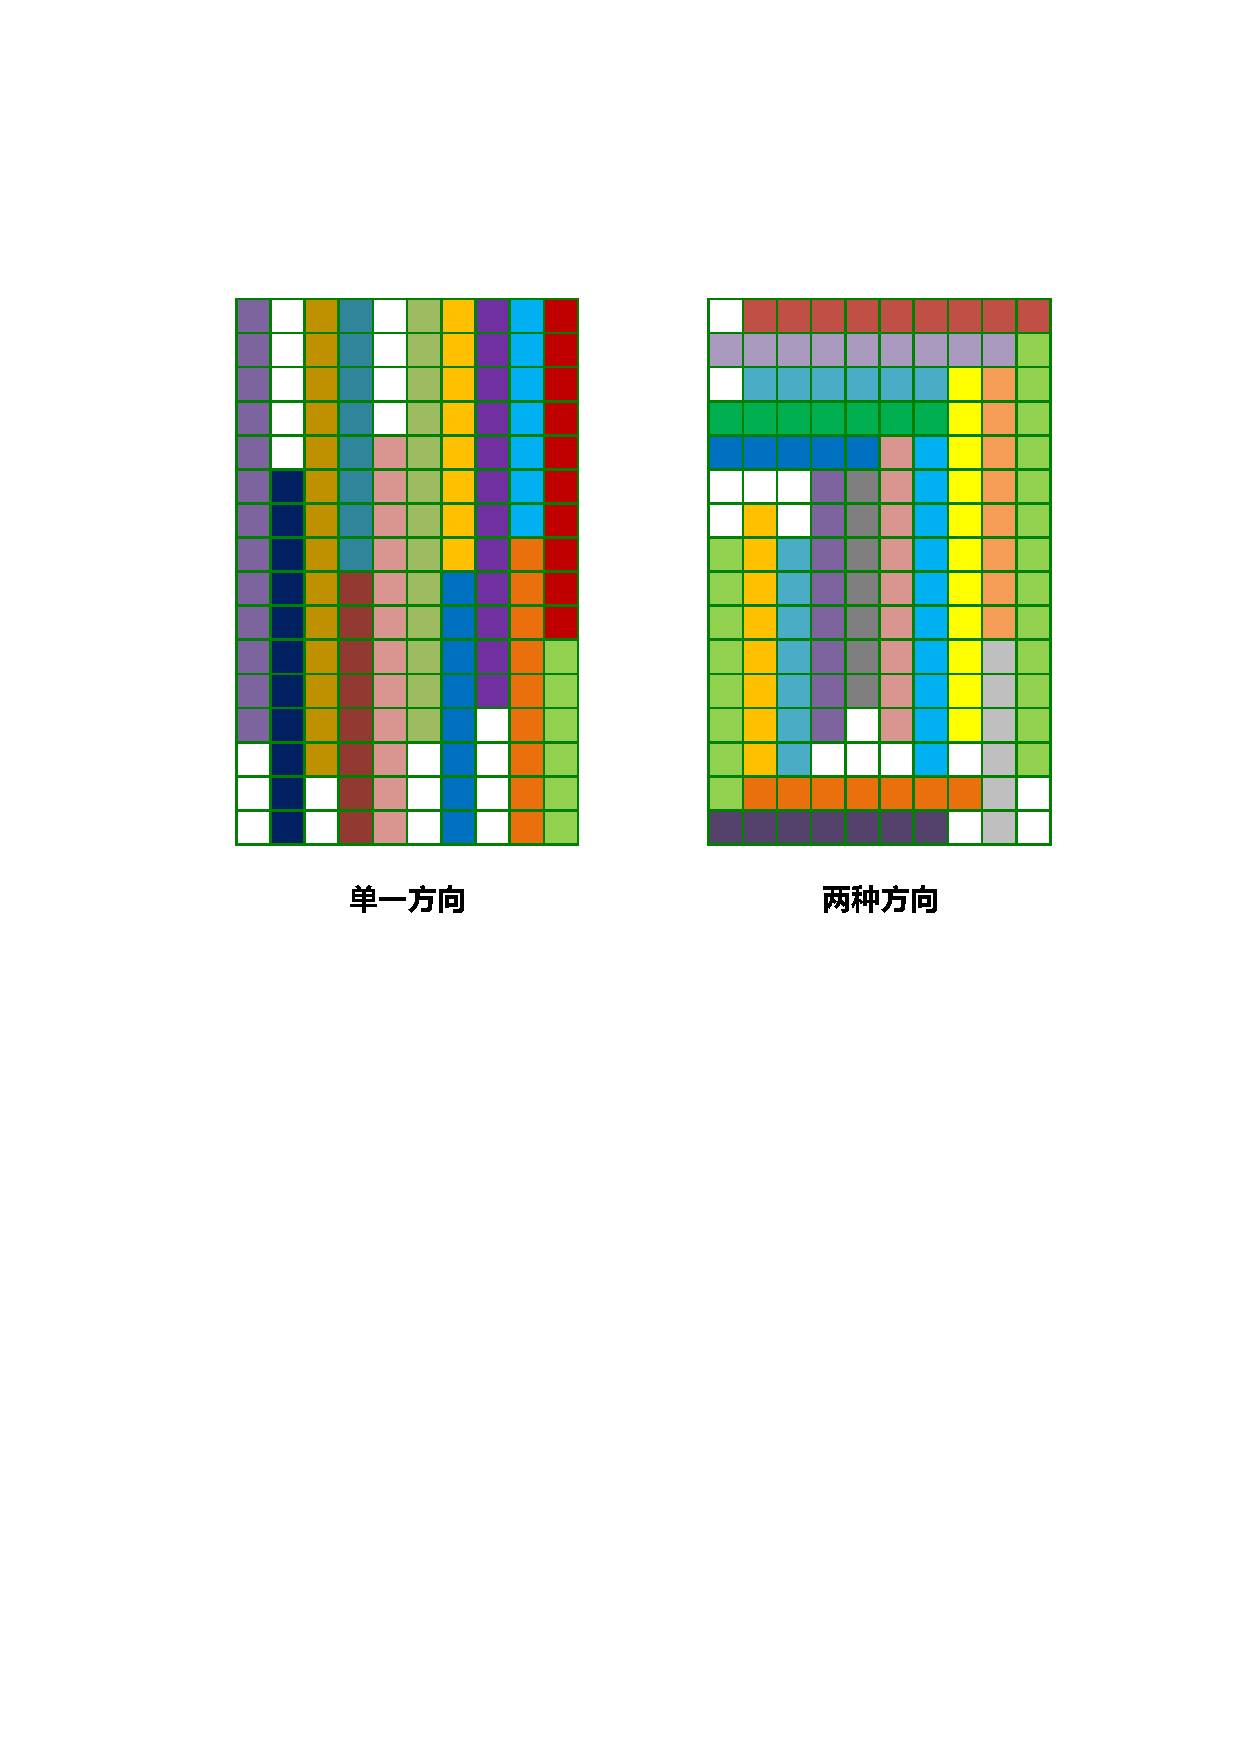
\includegraphics[width=0.8\textwidth]{Pictures/twoways.pdf}
\caption{两种在矩形天线阵列中放置天线子阵列的方案}
\label{fig:two}
\end{figure}

\section{单方向放置情况}
对于所有子阵列按照单一方向放置在天线矩阵中的情况,问题可以建模为:
\begin{equation}\label{eq:n1}
\begin{split}
&\max \,\, C_1 = \sum\limits_{k=1}^{K}\sum\limits_{i=1}^{I}\sum\limits_{j=1}^J p_{ij} x_{ijk}\\
&s.t.\quad  \left\{
\begin{array}{l}
\sum\limits_{i=1}^{I}\sum\limits_{j=1}^J l_{ij}x_{ijk}\leq L_k, ~ k=1,\dots,K,\\
\sum\limits_{j=1}^{J}\sum\limits_{k=1}^{K} x_{ijk}\leq 1,~ i=1,\dots,I,\\
x_{ijk}\in\{0,1\}, ~ i=1,\dots,I,j=1,\dots,J,
k=1,\dots,K,
\end{array}\right.
\end{split}
\end{equation}
其中 $x_{ijk}=1$ 代表用户$i$ 被分配了在$k$行的长度为$l_{ij}$的子阵列,否则为 $0$。 $p_{ij}$ 是用户 $i$ 被分配了 $j$长度的子阵列时的收益,无论其处于矩阵的哪一行。 $l_{ij} \leq L_k$。 第一个限制条件保证了一个用户被分配的子阵列的长度不会超过天线阵列每行的最大长度。第二个限制条件保证了一个用户只能最多在唯一一行被分配唯一长度的天线。


由于要同时考虑每个用户分配的子阵列天线数量以及每个子阵列在整个天线阵列中所处的位置,因此很难直接解决该子阵列分配问题。对此首先考虑原问题的一个简单的情况,原矩形阵列为一宽度为$1$的矩形,即所有的可用天线单元都在阵列的同一行上。由于不用考虑子阵列在每行上的分配问题,因此该简化版问题只需要考虑每个被分配的子阵列所占用天线个数。另外,该简化版问题的最优解也是原问题最优解的上界。则简化版问题可以建模为:
\begin{equation}
\label{eq:n2}
\begin{split}
&\max \,\, C_1^1 = \sum\limits_{i=1}^{I}\sum\limits_{j=1}^J p_{ij} x_{ij}\\
&s.t.\quad  \left\{\begin{array}{l}
\sum\limits_{i=1}^{I}\sum\limits_{j=1}^J l_{ij}x_{ij}\leq N,\\
\sum\limits_{j=1}^{J} x_{ij}\leq 1,\quad i = 1,\dots,I,\\
x_{ij}\in\{0,1\}, \quad  i=1,\dots,I, j=1,\dots,J \end{array}\right.
\end{split}
\end{equation}

此问题是一个多选择背包问题(MCKP),也是一个NP-hard问题,可以通过从一个已知的NP-hard问题(背包问题,Knapsack Problem)规约而证明。

一个典型的背包问题可以描述为:
\begin{equation}
\begin{split}
\label{eq:12}
&\max \,\, C_1^{'} = \sum\limits_{q=1}^{Q} p_{q} x_{q}\\
&s.t.\quad  \left\{\begin{array}{l}
\sum\limits_{q=1}^{Q} a_{q}x_{q}\leq W,\\
x_{q}\in\{0,1\}, \quad  q=1,\dots,Q,\end{array}\right.
\end{split}
\end{equation}
其中$p_q$ 和 $a_q$ 分别是$q$的收益和权重。如果$q$被选择,则$x_q=1$ ,否则为 $x_q=0$。$W$是背包的总容量。

典型的背包问题可以看做是问题(\ref{eq:n2})的一个特殊情况。当$Q=I$, $W=N$时,可以找到一个特例。对于 $\forall \bar j \in [1,...,J]$, $(p_q,a_q):=(p_{i\bar j},l_{i\bar j})$和$(p_{ij},l_{ij}):= (0,0)$ for $i = 1,...,I, j= 1,...\bar j-1,\bar j+1,...,J$,也就是说$p_q$ 和 $a_q$可以只能选择对应于用户$i$的唯一的一个值。则问题(\ref{eq:n2})中的第二个限制条件不会产生任何限制,因为可以对$i = 1,...,I, j= 1,...\bar j-1,\bar j+1,...,J$设置$x_{ij}=0$。因此可以证明原问题的一个特殊情况是一个背包问题。又因为 背包问题已经是一个众所周知的NP-hard问题,则问题(\ref{eq:n2})以及其一般性问题(\ref{eq:n1})都是NP-hard问题。

一个算法A被称作是一个 $(1-\varepsilon)$-近似算法,当对于问题 $\Pi$ 如果输入为(I, $\epsilon$)时, 则算法输出一个结果 $S_A$ 满足
\begin{equation}
S_A \geq (1-\epsilon)OPT(\Pi)
\end{equation}
如果这是一个最大化问题。


对于这个一维的子阵列分配问题,首先提出了一个启发式算法。通过逐步最大化权重方程以得到合适的子阵列分配方案。将权重方程设置为边缘收益$f(i,j)$,即每个天线单元所能带来的增益收益
\begin{equation}
f(i,j) = p_{ij}/l_{ij}.
\end{equation}

具体算法如算法(\ref{alg:11})所示。首先,对于每个用户$i$找到最大的权重$f({i}, \tilde j_{i})$,并将其存储到一个等待列表中。$\tilde i$ 代表最大权重的用户,其权重为$f(i,\tilde j)$ 且 $\tilde j_{\tilde i}$ 代表对应的子阵列长度序号。令$N'$ 代表可用天线数量。 当$N'>0$时,即此时仍有可用的天线单元待分配时,检查这个长度是否可以容纳对应的子阵列长度$l_{\tilde i \tilde j_{\tilde i}}$。如果可以,则将$l_{\tilde i \tilde j_{\tilde i}}$天线分配给用户$\tilde i$,并且令$x_{\tilde i \tilde j_{\tilde i}} = 1$。接着检查这个用户是否被分配过天线,如果是则将之前的分配取消掉并使$x_{\tilde i l_{\tilde i}} = 0$,减少可用天线存量$N' = N' - l_{\tilde i \tilde j_{\tilde i}} + l_{\tilde i}$,并更新用户$\tilde i$所占用的天线数量$l_{\tilde i}$;否则这个用户为第一次被分配,只需要减少天线存量$N'$并更新 $l_i$ 为 $l_{\tilde i \tilde j_{\tilde i}}$。这里要强调的是 ,并不需要丢放弃掉被分配天线子阵列的用户,而是将这类用户保留在列表中并更新其边际收益权重$f({\tilde i}, \tilde j_{\tilde i})$:

\begin{equation}
  f({\tilde i}, \tilde j_{\tilde i}) = \frac{f({\tilde i}, \tilde j'_{\tilde i}) - f({\tilde i}, l_{\tilde i})}{l_{\tilde i \tilde j_{\tilde i}}-l_{\tilde i l_{\tilde i}}}
\end{equation}
其中 $f({\tilde i}, \tilde j'_{\tilde i})$ 代表子阵列长度大于$l_{\tilde i}$的用户$\tilde i$的最大权重。当可用天线单元数量不足时,即 $l_{\tilde i \tilde j_{\tilde i}} > N'$,找到最大的权重$f({\tilde i}, N')$,将$N'$天线分配给该用户,并取$N'=0$。取消掉之前的分配方案。重复以上过程直到$N'=0$。这个算法返回$x_{ij}$,代表了每个用户被分配了多少个天线。此时即可完成一维的分配方案。由于每次循环至少分配一个天线单元,此算法最多运行$N$个循环。在每个循环中,找到最大的权重的用户并更新其权重,计算复杂度为$O(MN)$。因此该启发式算法的计算复杂度为$O(MN^2)$。

\begin{algorithm}
\caption{: \emph{单方向一维放置方案的启发式算法}} \label{alg:11}
{
\begin{algorithmic}[1]
\STATE{\textbf{初始化:}$x_{ij} = 0$ 对于 $i=1:M, j = 1:J$, $N' = N$, $l_i = 0$ 对于 $i = 1,...,M$, }
\FOR {$l_{ij} < N'$}
\STATE {$\tilde j_i = \arg \max f(i,j),\quad i= 1,...,M$\\}
\ENDFOR

\WHILE{$N' > 0$}
\STATE{$\tilde i, \tilde j_{\tilde i} = \arg \max{f(i,\tilde j)}$}
\IF {$l_{\tilde i \tilde j_{\tilde i}} \leq N'$}
\STATE {$x_{\tilde i \tilde j_{\tilde i}} = 1$}
\IF {$l_{\tilde i} = 0$}
\STATE {$N' = N' - l_{\tilde i \tilde j_{\tilde i}}, l_{\tilde i} = l_{\tilde i \tilde j_{\tilde i}}$}
%\STATE{$l_{\tilde i} = a_{(\tilde i \tilde j_{\tilde i})} $}
\ELSE
\STATE {$x_{\tilde i l_{\tilde i}} = 0, N' = N' - l_{\tilde i \tilde j_{\tilde i}} + l_{\tilde i}, l_{\tilde i} = l_{\tilde i \tilde j_{\tilde i}} $}
%\STATE {$N' = N' - \tilde j_{\tilde i} + l_{\tilde i}$}
%\STATE{$l_{\tilde i} = \tilde j_{\tilde i} $}
\ENDIF
\STATE{找到最大的增量收益$f({\tilde i}, \tilde j'_{\tilde i})$ 对于每个用户 $\tilde i$}
\ELSE

\STATE{$\tilde i = \arg \max f(i,N'),\quad i \in I$}

\IF {$l_{\tilde i} = 0$}
\STATE {$x_{\tilde i {N'}} = 1, l_{\tilde i} = N'$}
\ELSE
\STATE {$x_{\tilde i l_{\tilde i}+{N'}} = 1, x_{\tilde i l_{\tilde i}} = 0, l_{\tilde i} = l_{\tilde i} + N'$}
%\STATE {$x^C_{\tilde i l_{\tilde i}} = 0$}
\ENDIF
\STATE{$f({\tilde i}, \tilde j_{\tilde i}) = 0, N'=0 $}
%\STATE{$N'=0$}
\ENDIF
\ENDWHILE
\RETURN{ $x$\\}
 %terminate the algorithm.
\end{algorithmic} }
\end{algorithm}

在此基础上,可以进一步改进该启发式算法以得到子阵列按照相同方向分布在矩形阵列上的分配方案。如算法(\ref{alg:22})所示。其核心方法在于当一个用户分配到阵列上的某一行时就不再改变其所在阵列。因此当分配某一行阵列天线时,只需要搜索还未被分配的用户或是在暂时分配在该行的用户。

首先找到剩余可分配天线数量最多的行,以及权重最大的未分配用户或是已暂时分配在该行的用户。如果对应的子阵列天线单元数量小于等于可分配天线数量,则将该子阵列分配到该行,更新该行的可用天线单元数量,如果该用户分配过则取消之前的分配。接着计算该用户的新的增量权重。当可分配天线数量小于对应的子阵列天线数量时,对于未分配用户或分配在该行的用户,计算使用该行所有剩余可分配天线数量时的权重(若已分配在该行则需要与已分配天线数量合并计算)。将权重最大的用户对应的子阵列分配在该行,并将该行剩余天线数量置为0。重复此过程直到没有天线单元剩余。算法返回$x_{ij}$ 和 $y_{ij}$代表了天线子阵列阵列的分配方案。该算法最多需要$UL$次循环因为每次循环至少会分配一个天线单元。在每次循环中,找到最多可分配天线单元的行需要$O(U)$,找到最大权重用户并更新其权重需要最多$O(ML)$。因此该算法的计算复杂度为$O(MU^2L^2)$。

\begin{algorithm}
\caption{: \emph{单方向二维放置方案的启发式算法}} \label{alg:22}
\begin{algorithmic}[1]
\STATE{\textbf{Initialize:}$x_{ij} = 0$ 对于 $i=1:M, j = 1:J$ \\$y_{ij} = 0$ 对于 $i=1:M, k = 1:U$\\ $ l_i = 0$ for $i = 1:M$ \\$r_k = L$, 对于 $k = 1,\dots,U$}

\FOR {$l_{ij}< L$}
\STATE {$\tilde j_i = \arg \max f(i,j)$\\}
\ENDFOR
\WHILE{$\max( r_{\tilde k} ) > 0$}
\STATE{$r_{\tilde k} = \max{r}$}
\STATE{$\tilde i = \arg \max f(i,\tilde j)$, 对于 $i=\{i: y_{ik} = 0|| y_{i\tilde k} = 1,k=1:U\}, $}
\IF {$l_{\tilde i \tilde j_{\tilde i}} \leq r_{\tilde k}$}
\IF {$l_{\tilde i} = 0$}
\STATE {$x_{\tilde i \tilde j_{\tilde i}} = 1, y_{\tilde i \tilde k}=1, r_{\tilde k} = r_{\tilde k} - \tilde j_{\tilde i}, l_{\tilde i} = l_{\tilde i \tilde j_{\tilde i}}$}
\ELSE
\STATE {$x_{\tilde i \tilde j_{\tilde i}} = 1, x_{\tilde i l_{\tilde i}} = 0, r_{\tilde k} = r_{\tilde k} - \tilde j_{\tilde i},l_{\tilde i} = l_{\tilde i \tilde j_{\tilde i}}$}

\ENDIF
\STATE{找到每个用户 $\tilde i$的最大增量收益$f({\tilde i}, \tilde j'_{\tilde i})$ }

\ELSE
%\STATE{$l_{\tilde i} = a_{\tilde i \tilde j_{\tilde i}}$}
\STATE{$\tilde i = \arg \max f(i,r_{\tilde k})$, 对于 $i=\{i: y_{ik} = 0|| y_{i\tilde k} = 1,k=1:U\}, $}

\IF {$l_{\tilde i} = 0$}
\STATE{$x_{\tilde i r_{\tilde k}} = 1, y_{\tilde i \tilde k} =1, l_{\tilde i} = l_{\tilde i \tilde j_{\tilde i}}$}
%\STATE {$x^C_{\tilde i \tilde j_{\tilde i}} = 1, x^C_{\tilde i l_{\tilde i}} = 0, y^C_{\tilde i \tilde k}=1,r_{\tilde k} = r_{\tilde k} - \tilde j_{\tilde i},l_{\tilde i} = a_{\tilde i \tilde j_{\tilde i}}$}
%\STATE{Calculate the increasing marginal profit $f({\tilde i}, \tilde j_{\tilde i})$}
\ELSE
\STATE{$x_{\tilde i l_{\tilde i}+r_{\tilde k}} = 1, x_{\tilde i l_{\tilde i}} = 0, l_{\tilde i} = l_{\tilde i}+ r_{\tilde k}$}
\ENDIF
\STATE{$f({\tilde i}, \tilde j_{\tilde i}) = 0,  r_{\tilde k} =0 $}
\ENDIF
\ENDWHILE
\RETURN{ $x, y$\\}
\end{algorithmic}
\end{algorithm}


事实上,该MCKP问题还可以通过一个使用Dyer-Zemel算法的完全多项式时间的算法 \cite{bansal2004improved}解决。然而此算法只适合于 $\sum\limits_{j=1}^{J} x_{ij} =  1,\quad i = 1,\dots,I$ 的情况,也就是说每个用户必须被分配一种且只有一种长度的天线子阵列,因此需要为每个用户添加一个空的选项,即加入一个长度为零且收益为零的子阵列作为备选。则MCKP问题的解法如算法(\ref{alg:1})所示。

\begin{algorithm}
\SetAlgoLined{}
\caption{MCKP问题算法} \label{alg:1}
\textbf{初始化:}每个子阵列的收益 $p_{ij}$, 每个子阵列的长度 $l_{ij}$ 和总的可用天线数量 $N$\;
\Repeat{停止}{
丢弃所有被支配子阵列。在类$i$中随机将两个子阵列$(ij_1,ij_2)$组成一对,对于每一对子阵列,如果$l_{ij_1} \leq l_{ij_2}$ 而且 $p_{ij_1} \geq p_{ij_2}$,则 $ij_2$ 被 $ij_1$支配。一直重复此过程直到所有被支配的子阵列都被找到并丢弃\;
对于所有剩下的子阵列对$(ij_1,ij_2)$,求得其斜率$\gamma_{ij_1ij_2} = \frac{p_{ij_2}-p_{ij_1}}{l_{ij_2}-l_{ij_1}}$\;
令 $\gamma$ 为斜率 $\{\gamma_{ij_1ij_2}\}$的中位数,求得$a_i$, $b_i$ 和 $M_i(\gamma)$\;
$M_i(\gamma) = \arg \max \limits_{j\in J}{\{p_{ij} - \gamma l_{ij}\}}$,
$a_i = \arg \min \limits_{j\in M_i(\gamma)}{l_{ij}}$,
$b_i = \arg \max \limits_{j\in M_i(\gamma)}{l_{ij}}$\;
\uIf {$\sum\limits_{i=1}^{I}{l_{ia_i}} \leq N \leq \sum\limits_{i=1}^{I}{l_{ib_i}}$}
{$\gamma$ 是最优, $ W = \sum\limits_{i=1}^{I}{l_{ia_i}} $, $ P = \sum\limits_{i=1}^{I}{p_{ia_i}}$. 最优解 $z^* = P + \gamma(N - W)$,停止\;}
\uElseIf{$\sum\limits_{i=1}^{I}{l_{ia_i}} \geq N$}
{对于每一个符合$\gamma_{ij_1j_2} \leq \gamma$的对 ($ij_1,ij_2$),删除子阵列 $j_2$\;}
\ElseIf{$\sum\limits_{i=1}^{I}{l_{ib_i}} \leq N$}
{对于每一个符合$\gamma_{ij_1j_2} \geq \gamma$的对 ($ij_1,ij_2$),删除子阵列 $j_1$\;}
}
最优解$x^*$最多会出现两个分数变量$x_{aba}$ 和 $x_{ab'a}$,而且他们只会存在于同一个类中。否则不存在分数变量,$x^*$即为问题的最优解.
$P_1$ 是 $z^*$ 除去分数变量后的收益,
$P_2$ 是分数变量 $x_{aba}$ 的收益,
$P_3$ 是分数变量 $x_{ab'a}$的收益,
$P_0 = \max{(P_1,P_2,P_3)}$\;
$P_0 \leq P^* \leq 3P_0$\;
\ForEach{$p \in \{1,2,...,3P_0\}$}{
\eIf{$p_{(i+1)j} \leq p$}
{$F(i+1,p) = \min \{F(i,p), \min \limits_{j \in N_{i+1}} \{{w_{(i+1)j} + F(i,{p-p_{(i+1)j}}} \}\}$}
{$F(i+1,p) = F(i,p)$}
}
输出 $P^* = \max\{{p|F(m,p) \leq N}\}$,$x^*$。
\end{algorithm}

算法(\ref{alg:1})的输出是一个$\{x^*|x_{ij}=1\}$的集合。将对应的$p_{ij}$ 和 $l_{ij}$ 分别存储到一组新的集合$p_i$和$w_{i}$中。同时因为在下一个过程中序号$j$对于每个用户$i$来说不再改变,因此可以丢弃掉序号$j$。

至此,得到了一组收益最高的天线子阵列,在总天线数量不超过总可用数量的前提下,其收益和不小于$(1-\epsilon)$的最大收益值$OPT(\Pi)$。进而,试图将这些长度为 $w_i$,收益为$p_{i}$的子阵列集合安排进天线阵列中,保留其中收益最高的部分,丢弃掉由于容量原因不得不丢弃的收益较小的部分。该子问题可以建模为
\begin{equation}\label{eq:n3}
\begin{split}
&\max \,\, C_1^2 = \sum\limits_{i=1}^{I}\sum\limits_{k=1}^K p_{i} x_{ik}\\
&s.t.\quad  \left\{\begin{array}{l}
\sum\limits_{i=1}^{I} l_{i}x_{ik}\leq L_k, \quad k = 1,\dots,K,\\
\sum\limits_{k=1}^{K} x_{ik}\leq 1,\quad i = 1,\dots,I,\\
x_{ik}\in\{0,1\}, \quad  i=1,\dots,I, k = 1,\dots,K \end{array}\right.
\end{split}
\end{equation}
其中 $L_k$ 于问题(\ref{eq:n1})中类似,是第$k$行中总的可用天线数量,且对于 $k=1,\dots,K$. $x_{ik} = 1$,有 $L_k=L$。$x_{ik} = 1$代表子阵列 $i$ 被放置在第 $k$ 行,$0$则没有。

由于问题本身是NP-hard的,因此目的是得到一个近似的算法,保留其中收益最大的子阵列。算法的主要思想是将收益最低的那些子阵列放置在每行之间的交界点处,并最终丢弃这些子阵列使得不违反每行及整体天线容量的限制。提出的算法使用贪婪的策略,如算法(\ref{alg:3})所示:

\begin{algorithm}
\SetAlgoLined
\KwData{从算法(\ref{alg:1})中得到的子阵列集合}
\KwResult{将这些子阵列安置进矩形阵列中}
初始化\;
将整排天线平均的分成 $U$ 行,每行长度为 $L$, 即行间分割点位于 $L, 2L,...,(U-1)L$\;
设每行可用的天线为 $r_k$\;
$x_i = 0$, $r_0 = 0$, $r_k = L$\;
$A[\quad], j=1$ \;
\For{$k = 1,...,K$}{
$r_k = r_k - r_{k-1}$\;
\While{$r_k >0$}{
$\tilde i = \arg\max (p_i|x_i = 0)$\;
\eIf{$r_k - l_{\tilde i} \geq 0$ }{
$x_{\tilde i} = 1$ \;
$r_k = r_k - l_{\tilde i}$ \;
$\tilde i = A[j], j++$\;
}{
\While{$r_k > 0$}{
$\bar i = \arg\min (p_i|x_i = 0)$ ;\tcc*[f]{找到最小收益的子阵列}\\
$r_k = r_k - l_{\bar i}$\;
$x_{\bar i} = 1$\;
$\bar i = A[j], j++$\;
}
}
}
}
按照顺序 $A$ 将子阵列放置在每行中\;
丢弃处在行间分割点的子阵列\;
\caption{单一方向放置情情况下的子阵列放置的贪婪式算法}\label{alg:3}
\end{algorithm}

通过简单的方法就能在满足容量限制条件下,保留至少$1/2$的系统收益。首先,将从问题 (\ref{eq:n2})中得到的子阵列放在一个长度为 $L_k \times K$的单行天线阵列中。接着将整个单行天线阵列平均的分成$K$行。规定子阵列完全处于某一行时,归属于它所在的行;如果当一个子阵列跨过两行之间的交界时,则将他归属于较前的一行,同时认为此行的容量限制被打破。至此,所有子阵列就都属于且只属于一个固定的行,即使他们中的某些打破了每行的容量限制。基于本文的假设$l_{ij} \leq L_k$,每行都能至少保留一半的系统收益,即整体的天线阵列也能保留至少$1/2$的系统收益。具体来说,对于那些容量限制没有被打破的行,它们保持了所有的子阵列系统收益。另一方面,对于那些容量限制被打破的行,如果处在交界点的子阵列的收益大于本行其余的子阵列时,保留此子阵列并放弃其他的阵列,反之亦然。这样无论在任何情况,都能够在不打破容量限制的情况下保持至少$1/2$的系统收益。对每行都进行该操作后可以满足得到至少$1/2$的总系统收益。因此可以将问题(\ref{eq:n2})和问题(\ref{eq:n3})的结果合并,得到至少$1/2(1-\epsilon)$的最大系统收益。

\section{双方向放置情况}

一般来说,当使用同一个均匀线性阵的时候,发射/接受增益会随着波束方向与阵列中垂线的角度增大而减小\cite{han2015large},这主要是由于阵列的相对有效面积减小所造成的。因此,当天线数量一定的时候,适当的调整某些子阵列的朝向,使得与用户通信的波束方向更加接近于子阵列的中垂线方向,可以提高整个系统的表现。

在本章中,将会使用一些背包问题和装箱问题的技巧。给定矩形天线阵列的长边被定义为水平方向,短边定义为垂直方向。也就是说整个矩形天线阵列$R$被定义为长度为$L$,宽度为$K$的矩形。子阵列$i$的长度$a_i$为平行于水平方向的天线单元数量,宽度$b_i$为垂直于长度方向的天线单元数量。

在这种情况下,子阵列的选择问题可以看做是一个多选择背包问题和2D的条状装箱问题的组合。即需要考虑如何从可选子阵列集合中选出合适的子阵列子集,并将其合理地放置在大的巨型天线阵列中,使得所有子阵列都沿着矩阵的某一条边平行放置,所有的子阵列都不互相重合或者超出矩形阵列的边界。同时,子阵列的选择也受到每个用户只能选择一个长度子阵列这一条件的限制。这两个子问题,一个是只考虑容量限制,不考虑放置方法的背包问题;另一个是考虑放置方法的装箱问题;两个问题都是NP-hard的。因此为了在有效的时间内解决此问题,只能考虑类似于单方向放置问题的近似算法。首先,在所有的备选子阵列中,选出一个子集,此子集包含每个用户对应的唯一子阵列,同时保留最多的系统收益。之后再将该子集内的子阵列合理的放置在原来的矩形阵列中,保留其中最多的收益,丢弃掉那些收益较低的子阵列,以保证系统容量的限制不被破坏。两个子问题都利用合适的近似算法予以解决,最终即可得到有着最差性能保证的近似算法。

第一个子问题可以建模为
\begin{equation}\label{eq:n4}
\begin{split}
&\max \,\, C_2^1 = \sum\limits_{r=0}^{1}\sum\limits_{i=1}^{I}\sum\limits_{j=1}^J p_{ijr} x_{ijr}\\
&s.t.\quad  \left\{\begin{array}{l}
\sum\limits_{r=0}^{1}\sum\limits_{i=1}^{I}\sum\limits_{j=1}^J l_{ij}x_{ijr}\leq L\times K,\\
\sum\limits_{j=1}^{J}\sum\limits_{r=0}^{1} x_{ijr}\leq 1,\quad i=1,\dots,I,\\
x_{ijr}\in\{0,1\}, \quad  i=1,\dots,I,j=1,\dots,J,r=0,1,\end{array}\right.
\end{split}
\end{equation}
其中$x_{ijr} = 1$ 代表用户$i$被分配了方向为$r$的长度$j$的子阵列。 $r$ 是方向指示变量, $r=0$ 或者 $r=1$ 分别代表子阵列平行于天线矩阵的水平边或者垂直边。
为了解决此问题,首先要丢弃掉被主导的子阵列。对于一个相同的用户 $i$, $l_{ij0}=l_{ij1}$,如果 $p_{ij0} \leq p_{ij1}$,此时认为子阵列 ${ij0}$ 被子阵列 ${ij1}$主导,反之亦然。显然对于问题(\ref{eq:n4}),丢弃被主导的子阵列不会降低最终的最优结果。则问题(\ref{eq:n4})可以被规约成一个类似于问题(\ref{eq:n2})的MCKP问题,进而可以在$O(nm/\epsilon)$时间内得到一个$(1-\epsilon)$的近似解。

现在有了一组子阵列集合,其总长度等于总的可用天线数量,且总收益至少是$(1-\epsilon)$最大系统收益。需要将这些有固定方向的子阵列放置进天线阵列中,在既不互相重叠也不超过阵列边界的情况下尽可能保留最多的系统收益。这里引入 Steinberg's algorithm\cite{steinberg1997strip}, 提出一个将若干长方形安置进一个更大的矩形$R$中的近似算法,如果矩形$R$满足如下条件:
\begin{equation}\label{eq:n5}
a_L \leq u, b_L \leq v, 2S_L \leq uv-(2a_L-u)_+(2b_L-v)_+
\end{equation}
其中$(x)_+ = \max(x,0)$ 且
\begin{equation}
\begin{split}
& a_L  = \max_{1\leq i\leq l}{a_i},\\
& b_L = \max_{1\leq i\leq l}{b_i},\\
& s_i = a_ib_i \quad (1\leq i\leq l),\\
& S_L = \sum_{i=1}^l{s_i}.
\end{split}
\end{equation}
$a_i$ 和 $b_i$ 分别是子阵列 $i$ 的宽度和高度。 $u$ 和 $v$分别是矩形$R$的宽度和高度。

具体到的问题中,首先得到一个子阵列集合,其天线数量和为整个天线阵列的可用天线数量。之后沿着原天线矩阵$R$的一条边将原矩阵翻转,得到另一个相同的天线矩阵。将这两个天线矩阵沿着翻转边贴合在一起,就得到了一个原天线矩阵2倍的天线矩阵。则以下的条件会符合。
\begin{equation}\label{eq:n6}
\begin{split}
&  a_L \leq L, \\
&  b_L \leq K, \\
&  2S_L \leq 2LK-(2a_L-K)_+(2b_L-2L)_+ \\
or\quad & 2S_L \leq 2LK-(2a_L-2K)_+(2b_L-L)_+ .\\
\end{split}
\end{equation}
因此,根据Steinberg算法,总能将之前得到的子矩阵集合填进扩充后的天线矩阵中。

接着,需要在得到的子矩阵集合中找到合适的子矩阵集合放置回原天线矩阵中。算法的主要思想与单一方向放置情况类似:将子阵列分成几个可行的放置集合,并从中选出收益最大子集作为最终的选择。特别地,在本情况中子阵列中共有三类可行的放置集合,如图(\ref{fig:2rectangle})所示。其中第一类蓝色的子阵列集合完全在左边的长方形内,第二类绿色的子阵列集合完全在右边的长方形内,第三类红色的子阵列集合都正好穿过两个长方形的交界线。由于在长方形边界上的子阵列都肯定能可行的放置在一个完整的原阵列中,可以简单地选择三类中收益最大的那类作为最终的放置方案,则至少能够保证保留了$1/3$的总收益。

尽管上述算法能够得到至少 $1/3$ 的最大系统吞吐量,仍然需要进一步提高算法的效果。这里提出一个贪婪式算法(\ref{alg:4}),通过将剩余的收益最高的那些子阵列放置进原天线阵列,进一步提高算法的收益。

\begin{algorithm}
\SetAlgoLined
\KwData{从算法(\ref{alg:1})中得到的子阵列集合, $T$}
\KwResult{使原矩形阵列中收益最大的子阵列集合$T^*$}
将加倍后的矩形内的子阵列集合 $T$ 分成三类\;
找到 $T$ 中收益和最大的类 $T^*$  \tcc*[f]{其中包含至少 $1/3$ 的总系统收益}\;

\eIf {子阵列集合 $T^*$ 在一个原矩形阵列中} {返回}
{将子阵列集合 $T^*$ 平移放置在一个原矩形阵列中,可以证明一定能够通过平移放入一个原矩形阵列\;}
将剩下的子阵列集合 $\{T - T^*\}$ 按照收益降序排序 \tcc*[f]{将子阵列 $\{T-T^*\}$ 按照左先方式放置}\;
\For {当剩余可用空间大于子阵列集合 $T$中的最小子阵列所占长度时}{
在原矩形阵列中找到最大的可用矩形阵列R\;
\For{$j < size(\{T-T^*\}), j++$}
{
找到收益最大的子阵列 $t^* \in \{T-T^*\}$\;
\eIf{子阵列 $t^*$ 可以放置进R中}
{
按照左先下先方式放置子阵列 $t^*$ \;
$T^* = \{T^*,t^*\} $\;
}
{暂时移除$t^*$,直到有新的可用最大矩阵出现\;}
}}
返回: $T^*$
\caption{可互相垂直放置的情况下将加倍后的矩形阵列中的子阵列重新放置在原矩形阵列中的贪婪式算法。}\label{alg:4}
\end{algorithm}

\begin{figure}[htbp]
\centering
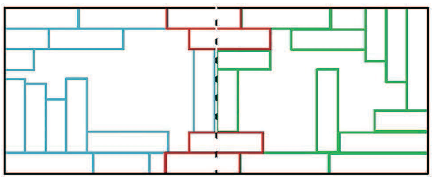
\includegraphics[width=0.7\textwidth]{Pictures/2rectangle.pdf}
\caption{加倍长方形中三类不同的子阵列状态}
\label{fig:2rectangle}
\end{figure}

\section{仿真验证}

在本章中,展示了不同场景下提出的两种算法的性能评价。仿真实验均在一台频率为3.2GHz的Intel\textregistered  ~Core\texttrademark ~ i5-4570 CPU的计算机上,利用MATLAB\textregistered 实现。
\begin{figure}[htbp]
\centering
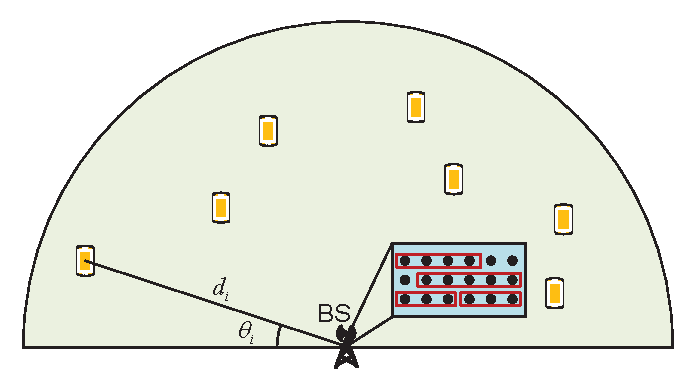
\includegraphics[width=0.7\textwidth]{Pictures/tu33}
\caption{毫米波通信天线资源优化调度仿真场景}
\label{fig:310}
\end{figure}

天线阵列是一个$K \times L$的长方形阵列。通信频率使用60GHz,两个相邻天线之间的距离为半波长,即2.5毫米。小区认为是个圆形小区,天线阵列位于被放置圆心处的基站上。如图(\ref{fig:310})所示,BS代表基站,蓝色的长方形代表大规模天线阵列,黑色点代表天线单元,每一个红色框中的天线代表一个天线子阵列与一个用黄色手机代表的用户进行通信。用户的位置用距离$d_i$和角度$\theta_i$来描述。用户随机的分布在角度为 $\theta_i \in (-90^{\circ}, 90^{\circ})$的半圆上,到圆心的距离为$d_i \in [10m, 50m]$。对于每个用户,目标方向即为其自身所处方向$\theta_i$。加性噪声为零均值的高斯过程$\mathbf{n}(t)\sim CN(0,\sigma_n^2 \mathbf{I})$。使用\cite{carlson1988covariance}中的模拟滤波算法来计算式~\eqref{eq:1}中的权重向量$\mathbf{w}$。则收益$p_{ij}$可以通过式~\eqref{eq:3}得到。

首先我们比较了在单方向放置情况下的一维与二维启发式放置方案的性能比较。

\begin{figure}[htbp]
    \centering
    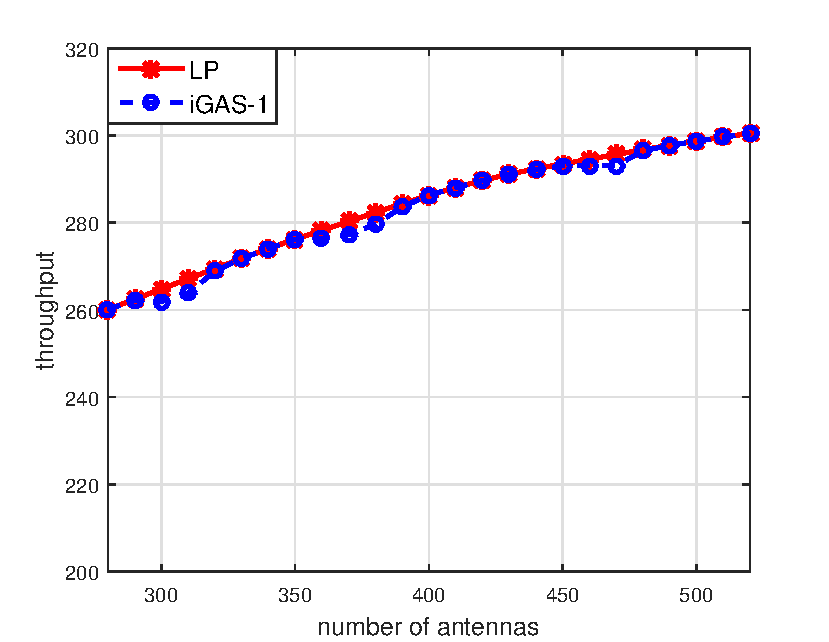
\includegraphics[width=0.7\textwidth]{Pictures/11}
    \caption{不同天线数量下的线性规划与一维启发式算法性能比较}
    \label{fig:111}

\end{figure}

\begin{figure}[htbp]
    \centering
    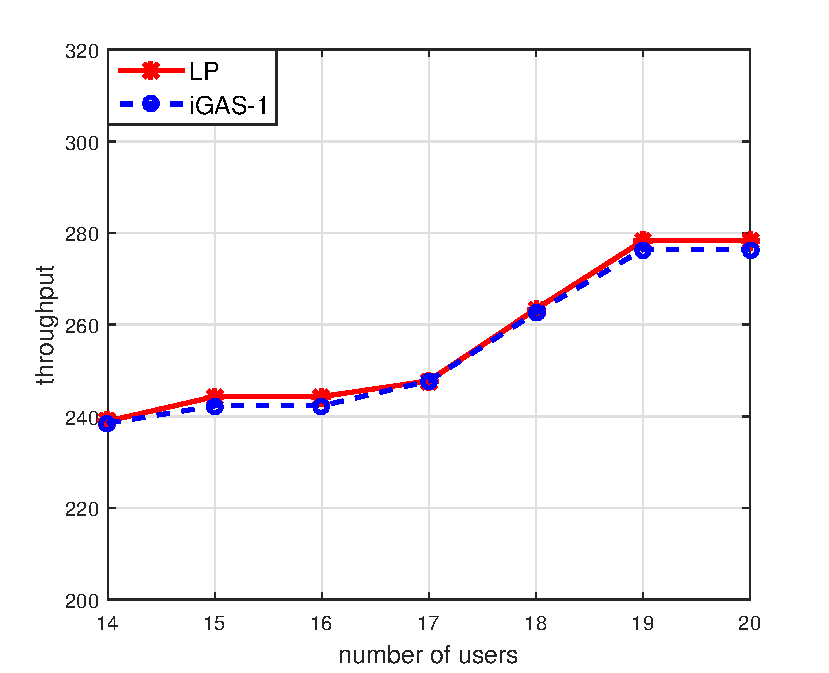
\includegraphics[width=0.7\textwidth]{Pictures/22}
    \caption{不同用户数量下的线性规划与一维启发式算法性能比较}
    \label{fig:222}

\end{figure}

\begin{figure}[htbp]
    \centering
    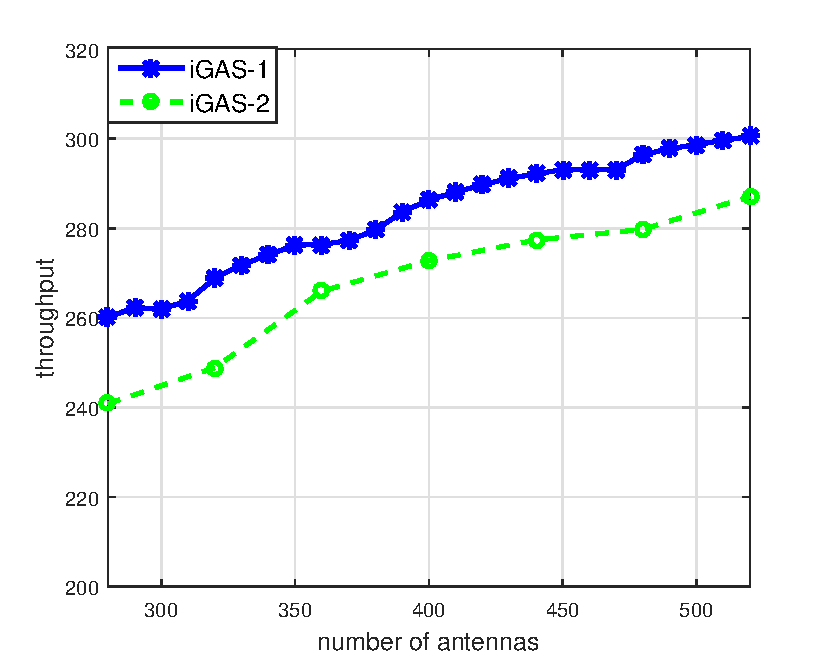
\includegraphics[width=0.7\textwidth]{Pictures/33}
    \caption{不同天线数量下的一维与二维启发式算法性能比较}
    \label{fig:333}

\end{figure}
\begin{figure}[htbp]
    \centering
    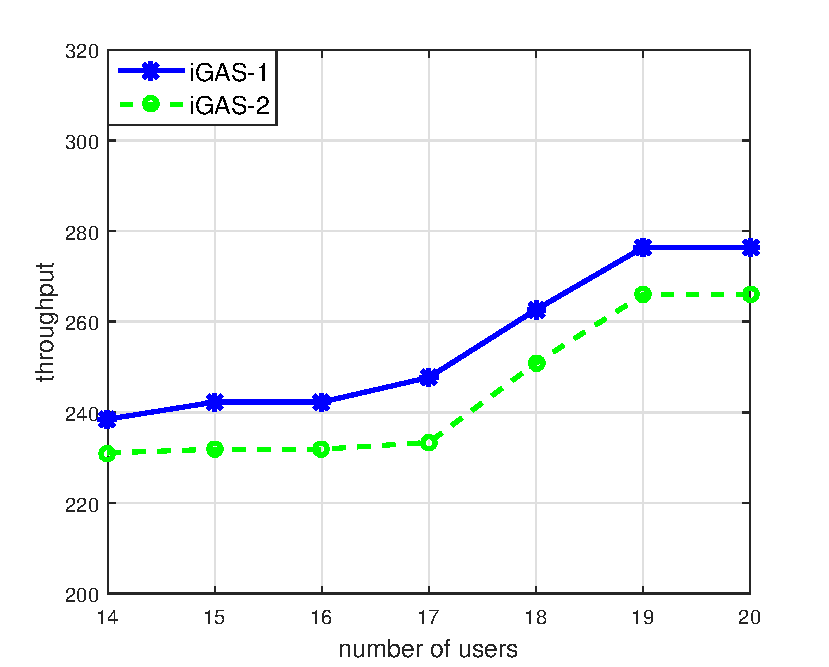
\includegraphics[width=0.7\textwidth]{Pictures/44}
    \caption{不同用户数量下的一维与二维启发式算法性能比较}
    \label{fig:444}
\end{figure}


图(\ref{fig:111})展示了不同天线数量下的线性规划与一维启发式算法性能比较。LP代表了线性规划的性能,iGAS-1代表了一维启发式算法性能。该场景中共有20个用户,总天线单元数量从280增加到520。吞吐量的单位为Mbps。很明显随着天线单元数量的增多,提出的一维启发式算法性能逐渐提高,且几乎能得到与线性规划类似的系统性能。

图( \ref{fig:222})展示了不同用户数量下的线性规划与一维启发式算法性能比较。与上图类似,总天线单元数量设置为360,用户数量从14增加到20。显然在一定用户数量范围内,当用户数量增加时,系统性能逐渐增长,所提出的一位启发式算法与线性规划算法能够得到相近的系统性能。

图( \ref{fig:333})展示了不同天线数量下的一维与二维启发式算法性能比较。 iGAS-1和iGAS2分别代表了一维与二维启发式算法。用户数量设置为20个,天线数量从280增长到520.由于对于二维启发式算法来说很难得到理论上界,这里使用一维的性能表现与二维算法做比较。与预期相同,二维算法的性能与一维启发式算法相比较差,其原因在于在一维情况下可以分配给用户的子阵列在二维情况下由于形状的限制,不能进行分配,只能选取次优的选择。从图中可见随着天线单元数量的提升,iGAS算法的性能逐渐提高,且两个算法间的性能差距约为$ratio = \frac{performance(iGAS-2)}{performance(iGAS-1)}\approx 0.93$。

图( \ref{fig:444})给出了不同用户数量下的一维与二维启发式算法性能比较。天线单元数量设置为360,用户数量从14增加到20个。显然在一定用户数量范围内,随着用户数量的增加,两个算法的系统性能表现都逐渐增加,且两者之间的的性能差距基本保持不变。

\begin{figure}[htbp]
\centering
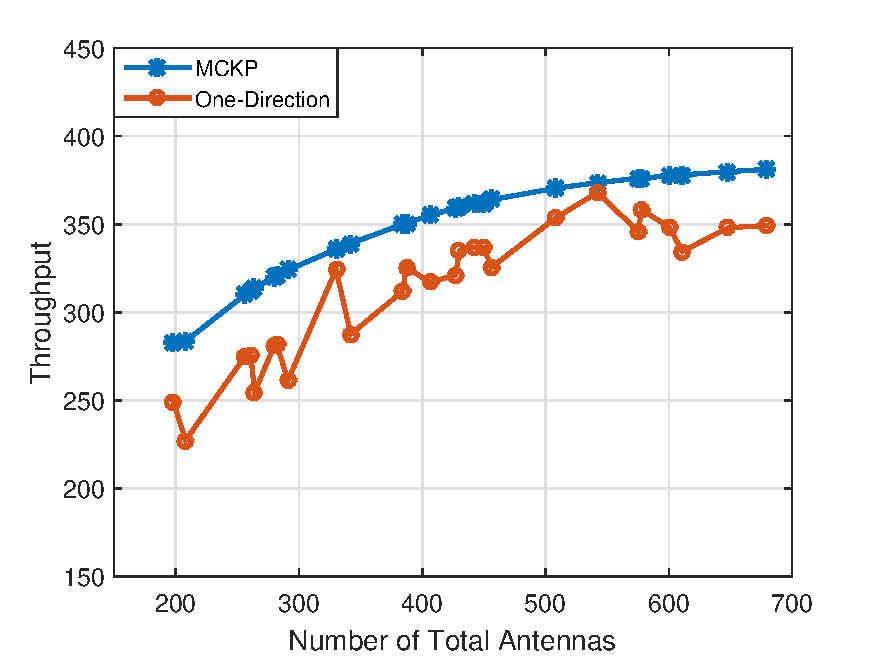
\includegraphics[width=0.7\textwidth]{Pictures/fig66}
\caption{总可用天线数量不同时两种算法的系统吞吐量比较}
\label{fig:2}
\end{figure}

\begin{figure}[htbp]
\centering
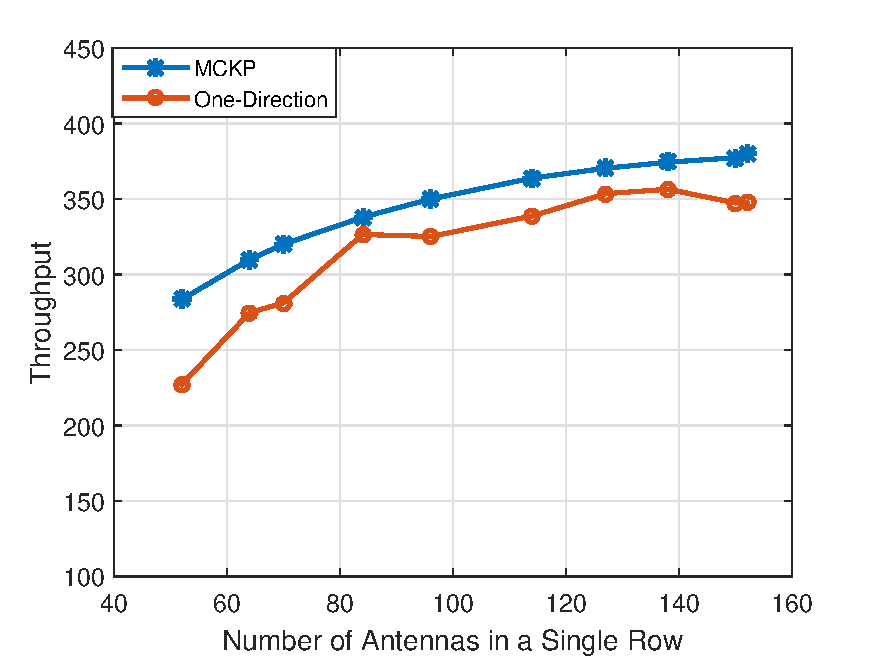
\includegraphics[width=0.7\textwidth]{Pictures/fig88}
\caption{天线矩阵行数不变(4行),每行天线数量不同时两种算法的系统吞吐量的比较}
\label{fig:4}
\end{figure}

\begin{figure}[htbp]
\centering
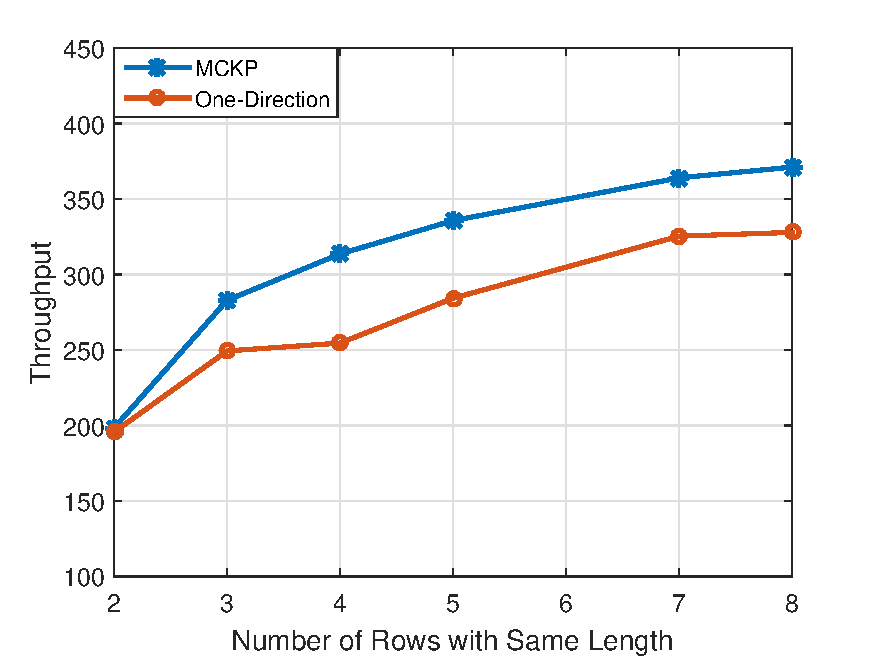
\includegraphics[width=0.7\textwidth]{Pictures/fig99}
\caption{每行可用天线数量不变,天线行数不同时两种算法的系统吞吐量的比较}
\label{fig:5}
\end{figure}

之后测试基于MCKP的两种算法性能表现。图(\ref{fig:2})展示了总天线数量变化时算法(\ref{alg:3})及其上界MCKP算法的性能比较。共有$20$个用户随机分布在半圆形的小区内,其中基站天线阵列位于圆心的位置。如图所示, MCKP算法的性能表现随着可用天线数量的增多而上升;同时算法(\ref{alg:3})的性能有着相同的趋势的同时,产生了一些波动。这些波动的来源主要是由每行天线数量的不同所造成的。虽然总的天线数目一直在增加,但是由于天线阵是一个矩形阵列,由于行数的增加,每一行上的天线数量可能减少,这就限制了每一行上天线子阵列放置的自由度。一般来说,每一行上的可用天线越多,子阵列的选择就越多,系统的性能就越好。因此,随着总天线数量的增加,算法的表现是在波动中上升。

图(\ref{fig:4})展示了在总行数不变(保持4行)的情况下,每行可用天线数量与两个算法性能之间的关系。可以明显的看到两个算法的性能都随着天线数量的增加而提高。算法之间的性能差异在某些时刻会突然减小,这一般是因为在这些情况下,理论上最优的子阵列分割策略正好与行之间的切换点相吻合,只有很少的一部分收益低的子阵列会被丢弃掉,系统得以保留更多的收益。此时,算法的性能几乎可以与理论最优值相媲美。

在图(\ref{fig:5})中,研究了当每行天线数量不变(每行66个可用天线)而总行数改变时的算法性能。很明显由于增加了更多的可用天线,增加行数能够提高总的系统吞吐量。可以发现随着行数的增多,性能的提升效果逐渐降低,这是由于随着天线数量的上升,之前行中的收益逐渐饱和,只有那些收益较低的子阵列会在新的行中保留。

\begin{figure}[htbp]
\centering
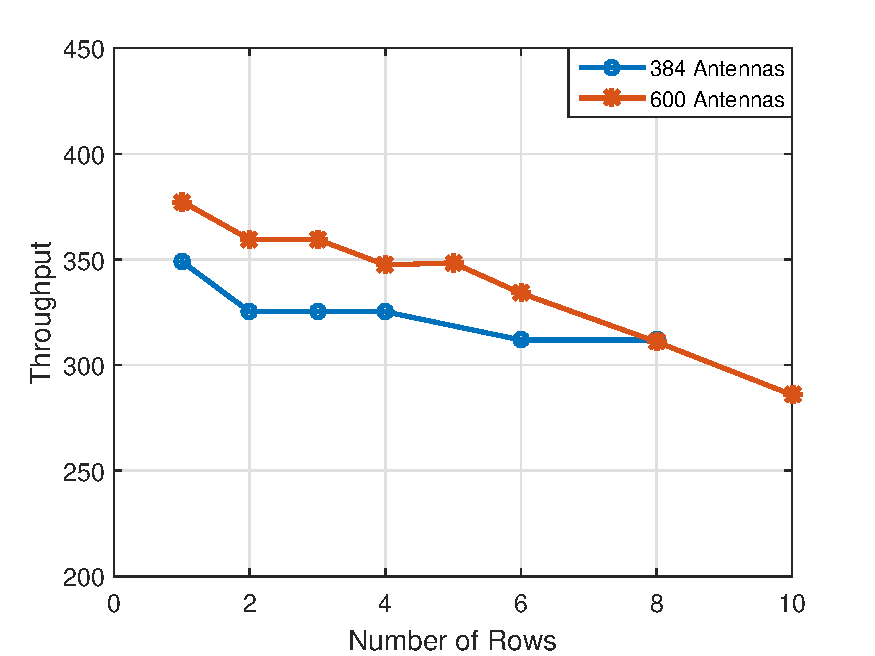
\includegraphics[width=0.7\textwidth]{Pictures/fig77}
\caption{当总天线数量固定,每行天线单元个数改变时两种算法的系统吞吐量比较}
\label{fig:3}
\end{figure}

\begin{figure}[htbp]
\centering
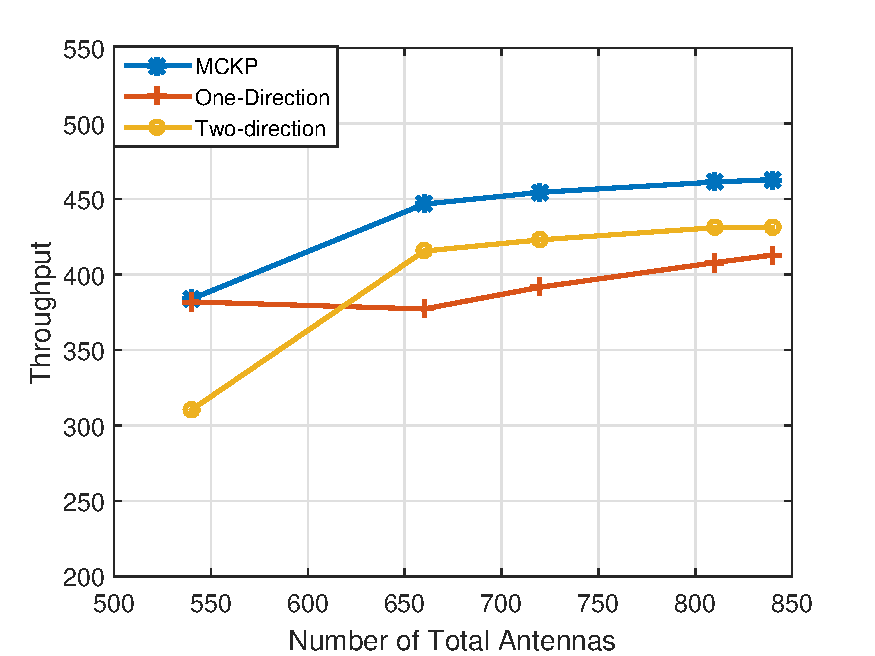
\includegraphics[width=0.7\textwidth]{Pictures/3compare}
\caption{三种算法在天线单元数量不同时的系统吞吐量比较}
\label{fig:6}
\end{figure}


\begin{figure}[htbp]
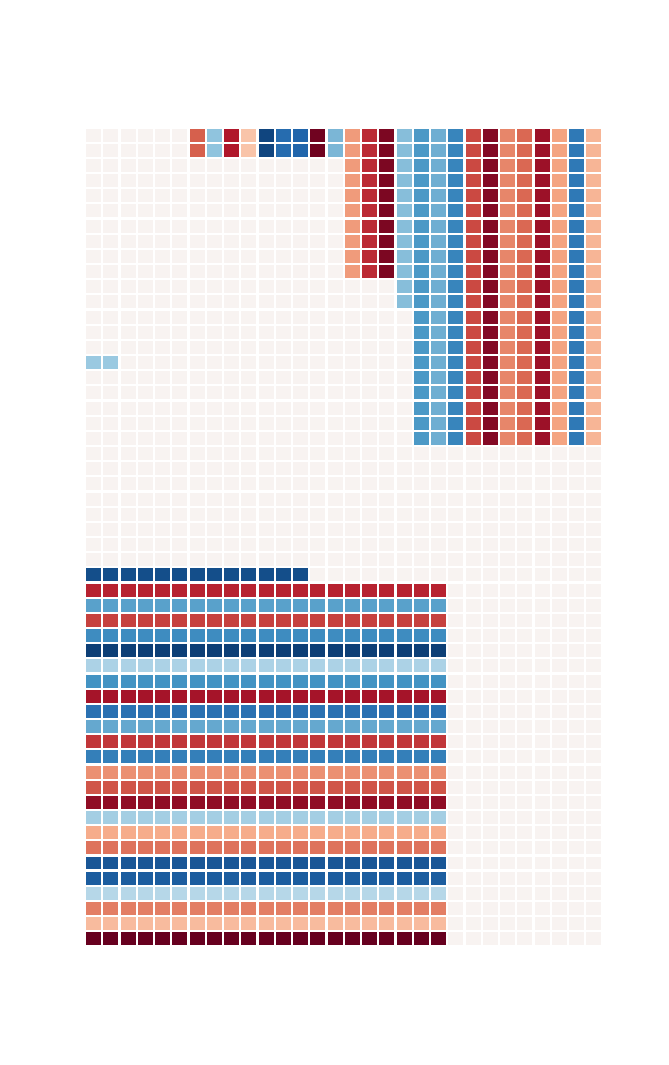
\includegraphics[width=0.8\textwidth]{Pictures/figure_1}
\centering
\caption{在加倍后的天线阵列中天线子阵列的放置结果示意图}
\label{fig:311}
\end{figure}

\begin{figure}[htbp]
\centering
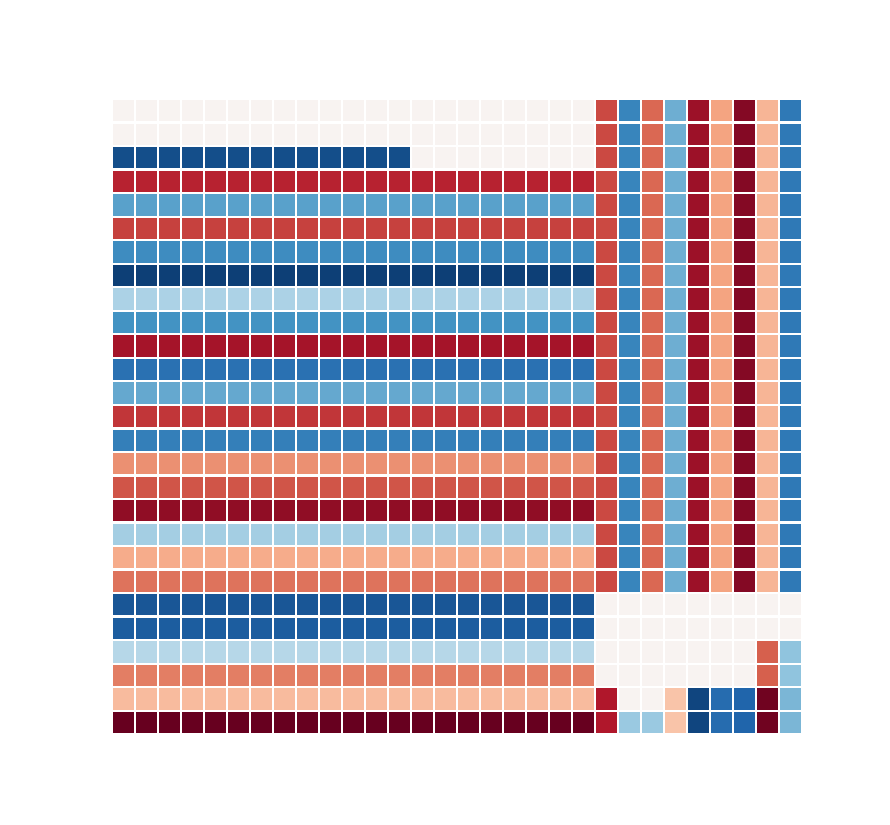
\includegraphics[width=0.8\textwidth]{Pictures/figure_0}
\caption{在原天线阵列中天线子阵列的放置结果示意图}
\label{fig:312}
\end{figure}

图(\ref{fig:3})展示了当总的天线数量固定,但每行的天线数量于总天线行数变化时算法(\ref{alg:3})的效果。由于行数的增加,每行的最大可用天线数量逐渐减少,因此可允许的子阵列的自由度也相应减小,因此可以观察到当总天线数量一定时,系统性能随着行数的增加而降低。

在图(\ref{fig:6})中比较了单排列方向和双排列方向两种情况。可以看出两种情况下的算法都能够得到很好的表现。当天线数量较少时,单方向情况的算法略微优于双方向情况,其主要原因在于较少的天线数量限制了两个方向上的最大天线数量,进而限制了子阵列放置的自由度。当总的天线数量增加时,两个方向上的天线最大数量增加,于是更换子阵列方向的优势得以体现。

图(\ref{fig:311})给出了如何将线性子阵列分布在加倍后的天线阵列中。每个小方块代表一个天线终端,每一个颜色代表一个与用户通信的子阵列,未涂色方块代表未使用的天线。原天线阵列为 $27\times30$ 的矩形天线阵列,共包含$810$个天线。根据所提出的算法,将原阵列扩充成一个$54\times 30$的阵列。首先通过MCKP算法选出总天线数量为$810$的备选子阵列,之后将此子阵列放入双倍扩充后的天线矩阵中。图(\ref{fig:312}) 给出了在图(\ref{fig:311})的基础上,利用贪婪算法重新放置后的分配图。备选子阵列集合中收益最大的子阵列集合被保留了下来,提高了天线资源利用率。

\section{本章小结}

本章研究了毫米波通信应用在蜂窝小区这一典型星型网络场景中的资源优化分配问题,即蜂窝小区基站上大规模多输入多输出系统天线子阵列选择问题,目的是最大化系统吞吐量。问题按照不同的天线子阵列放置方法分为两种情况:1)所有线性子阵列同一方向放置,2)为了进一步提升系统吞吐量,线性子阵列可以相互垂直方向放置。针对这两个NP-hard问题,首先对于单方向情况提出了启发式算法解决方案,之后进行问题分解,依次解决了一个多选择背包问题和一个多背包问题,并求得一个$1/2(1-\epsilon)$-近似的算法。接着对于垂直方向放置的情况进行问题分解,依次解决了一个多选择背包问题和一个二维带状装箱问题,并最终提出一个$1/3(1-\epsilon)$-近似的解法。两种算法在其各自场景中都能得到很好的效果,仿真结果验证了算法的有效性。在研究了星型网络场景后,下一章将研究在无线数据中心网络这一网状网络场景下的毫米波通信资源优化分配问题。
